
\section{Einführung}
\label{einleitung_sec}

Thema des Projektpraktikums \emph{Kognitive Automobile} ist es, eine virtuelle Test- und Simulationsumgebung für reale Erprobungsfahrten in einem autonomen Fahrzeug zu erzeugen.
Dies geschieht unter Zuhilfenahme einer 3D-Augmented-Reality-Brille mit Inertialsensorik, welche in den \ac{FZI}-Versuchsträger CoCar integriert wird.


\subsection{Motivation}
\label{einleitung_motivation_subsec}


Neuentwicklungen im Bereich des autonomen Fahrens müssen ausgiebig getestet werden, bevor sie in Fahrzeugen Anwendung finden können.
Rein virtuelle Simulationen sind zum Testen ein geeignetes Mittel, sie geraten jedoch häufig an ihre Grenzen.
Daher ist es in der Entwicklung von autonomen Fahrfunktionen unerlässlich, diese auch im realen Fahrbetrieb zu testen.

In bestimmten Szenarien (beispielsweise eine Notbremsung aufgrund eines Fußgängers oder autonomes Einparken im Parkhaus) ist Testen in der Realität allerdings gefährlich.
Das Risiko, einen Passanten zu verletzen bzw. mit der teuren Versuchsplattform gegen die Parkhauswand zu stoßen, kann nicht eingegangen werden.

Für solche Fälle ist eine hybride Umgebung, bestehend aus realer Versuchsplattform und simulierter Umgebung, ein möglicher Ansatz.
Der Sicherheitsfahrer bekommt dazu simulierte Hindernisse in der \ac{AR}-Brille eingeblendet und kann die Reaktion des Autos in der Realität überwachen.

Die Anwendung einer solchen \ac{AR}-Brille kann ebenso zur Einblendung von weiteren Daten wie beispielsweise aktuellen Manöver-, Navigations- oder Entertainment-Informationen verwendet werden.

%Was ist damit?  --> siehe commit-comment 77d294a54
%Im Kontext Kognitiver Automobile hat eine Kalibrierte 3D Sicht ebenfalls eine große Bedeutung: Hierbei gibt es zwei große Anwendungsgebiete, einerseits können hiermit neue Geräte oder Anzeigen Simuliert werden, andererseits kann hiermit aber auch eine Simulierte Realität dem Sicherheitsfahrer angezeigt werden. So wird z.B. ein Auffahrbremsen simuliert, so kann dem Fahrer das Simulierte Auto angeziegt werden. Oder wird in eine simulierte Parkbuch eingeparkt, so kann diese vom Sicherheitsfahrer durhc die Brille beurteilt werden.


\subsection{Aufgabenstellung}
\label{einleitung_aufgabenstellung_subsec}


In diesem Projektpraktikum soll ein wie in Abs.~\ref{einleitung_motivation_subsec} beschriebenes hybrides System entwickelt werden.

Die wesentlichen Komponenten für eine solche \ac{AR}-Umgebung sind:
\begin{itemize}
  \item Headtracking zur Bestimmung der Kopforientierung
  \item Augenbezogene Einblendung von Objekten
\end{itemize}

Für die Bestimmung der Kopforientierung soll primär die Inertialsensorik der \ac{AR}-Brille verwendet werden.
Die Kompensation der Eigenbewegung des Fahrzeugs ist unter Zuhilfenahme weiterer Sensorik zu bewältigen.
Zur Verfügung stehen die Inertialsensorik des Autos, die im Auto verbaute Kinect-Sensorleiste sowie die direkt auf der \ac{AR}-Brille montierte Kamera.

Des Weiteren soll untersucht werden, wie eine augenbezogene Einblendung von Objekten in das Sichtfeld des Fahrers mittels der \ac{AR}-Brille ermöglicht werden kann.
Dafür ist zum einen eine Auge-Display-Kalibrierung vorzunehmen.
Zum anderen sollen anzuzeigende Objekte für eine 3D-Einblendung aufbereitet werden (Stereoskopisches 3D).


\subsection{Hard- und Software}
\label{einleitung_hardware_subsec}

Für die beschriebene Aufgabenstellung steht als Hardware eine \ac{AR}-Brille des Herstellers \emph{Vuzix} vom Typ \emph{Star 1200} zur Verfügung, s.~Abb.~\ref{fig:vuzix_star_1200}.
Diese besitzt folgende Merkmale:
\begin{itemize}
  \item Zwei vor den Augen angebrachte transparente Displays (Blickwinkel ca. $30^\circ$)
  \item Eine feste Kamera (Logitech Webcam)
  \item \ac{IMU} (\emph{Wrap Tracker 6TC}), bestehend aus zwei Gyroskopen, einem Beschleunigungssensor sowie einem Magnetometer
\end{itemize}

\begin{figure}[h]
  \centering
  %\missingfigure{Vuzix}
  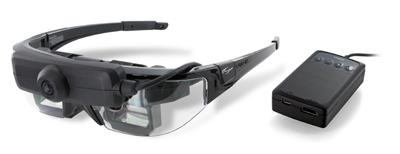
\includegraphics[width=0.4\textwidth]{vuzix}
  \caption{\ac{AR}-Brille \emph{Vuzix Star 1200}\ \cite{vuzix}}
  \label{fig:vuzix_star_1200}
\end{figure}

Für die Programmierung stehen die \ac{ICL}-Softwareumgebung des \ac{FZI}, sowie das \ac{ROS}-Framework \cite{ros} zur Verfügung.
